% AP Statistics Video Follow-Along Worksheet
% Unit 3, Lesson 5: Introduction to Experimental Design (Videos 1-3)

\documentclass[11pt]{article}
\usepackage[margin=0.85in, headheight=14pt]{geometry}
\usepackage{enumitem}
\usepackage{amsmath}
\usepackage{amssymb}
\usepackage{fancyhdr}
\usepackage{tcolorbox}
\usepackage{array}
\usepackage{booktabs}
\usepackage{xcolor}
\usepackage{tikz}

% Define colors
\definecolor{apblue}{RGB}{0, 51, 102}
\definecolor{lightgray}{RGB}{245, 245, 245}
\definecolor{boxborder}{RGB}{180, 180, 180}

% Header setup
\pagestyle{fancy}
\fancyhf{}
\lhead{AP Statistics}
\chead{Unit 3: Collecting Data}
\rhead{Lesson 3.5}
\lfoot{Name: \underline{\hspace{2.5in}}}
\rfoot{Period: \underline{\hspace{0.75in}}}

% Custom box environments
\tcbset{
    vocabbox/.style={
        colback=lightgray,
        colframe=boxborder,
        boxrule=1pt,
        arc=3pt,
        left=8pt,
        right=8pt,
        top=6pt,
        bottom=6pt
    },
    objectivebox/.style={
        colback=white,
        colframe=apblue,
        boxrule=1.5pt,
        arc=3pt,
        left=8pt,
        right=8pt,
        top=6pt,
        bottom=6pt
    }
}

% Blank line command
\newcommand{\blank}[1]{\underline{\hspace{#1}}}

\begin{document}

% Title
\begin{center}
    {\Large \textbf{Topic 3.5: Introduction to Experimental Design}}\\[4pt]
    {\large \textit{How do we design studies that can establish causation?}}\\[8pt]
    \textbf{Video Follow-Along Worksheet (Videos 1--3)}
\end{center}

\vspace{0.3em}

% Learning Objective Box
\begin{tcolorbox}[objectivebox]
\textbf{Learning Objectives:}
\begin{itemize}[leftmargin=1em, topsep=2pt, itemsep=1pt]
    \item \textbf{VAR-3.A:} Identify the components of an experiment.
    \item \textbf{VAR-3.B:} Describe the elements of a well-designed experiment.
    \item \textbf{VAR-3.C:} Compare experimental designs and methods.
\end{itemize}
\vspace{4pt}
\textbf{Essential Knowledge:} Well-designed experiments can establish evidence of causal relationships through comparisons, random assignment, replication, and control of confounding variables.
\end{tcolorbox}

\vspace{0.5em}

% Vocabulary Box
\begin{tcolorbox}[vocabbox, title={\textbf{Key Vocabulary}}]
\begin{tabular}{@{}p{1.5in}p{4.2in}@{}}
\textbf{Experiment} & A study where treatments are intentionally imposed on experimental units to observe a response. \\[3pt]
\textbf{Experimental units} & The individuals (people, animals, objects) to which treatments are applied. \\[3pt]
\textbf{Confounding variable} & A variable related to the explanatory variable that also influences the response, creating a false perception of association. \\[3pt]
\textbf{Random assignment} & Using chance to determine which treatment each experimental unit receives. \\[3pt]
\textbf{Placebo} & A ``fake'' treatment similar in appearance to the real treatment. \\[3pt]
\textbf{Blinding} & When subjects and/or researchers do not know which treatment is being administered.
\end{tabular}
\end{tcolorbox}

\vspace{0.75em}

%==============================================================================
% VIDEO 1
%==============================================================================

\section*{\underline{Video 1}: Confounding \& Components of an Experiment \hfill \normalfont\small [6:20]}

\subsection*{Part A: The Problem with Observational Studies \hfill \normalfont\small [0:00--3:12]}

\begin{enumerate}[label=\arabic*., leftmargin=2em]
    \item \textbf{Research question:} Do students who take notes during AP Stats earn \blank{1.25in} than students who just listen?
    
    \vspace{0.3em}
    
    \item One way to study this is through an \blank{2in}: observe student grades after the midterm and record which students regularly took notes.
    
    \vspace{0.3em}
    
    \item If the group who took notes earned higher grades, can we conclude taking notes \textit{caused} the higher scores?
    
    \hfill \textbf{Circle one:} \quad Yes \quad / \quad No
    
    \vspace{0.3em}
    
    \item Just because there's a \blank{1.25in} does not automatically mean there's \blank{1.25in}.
    
    \vspace{0.3em}
    
    \item A \textbf{confounding variable} is another variable that is related to the \blank{1.75in} variable and influences the \blank{1.5in} variable.
    
    \vspace{0.3em}
    
    \item In this example, \blank{2in} is a confounding variable because:
    \begin{itemize}[leftmargin=1.5em, topsep=2pt]
        \item Students who are academically motivated are more likely to \blank{1.5in}.
        \item Students who are academically motivated are more likely to \blank{1.5in}.
    \end{itemize}
\end{enumerate}

\vspace{0.4em}

% Causal Diagram
\begin{tcolorbox}[colback=white, colframe=apblue, boxrule=1pt, title={\textbf{Confounding: Visualized}}]
\begin{center}
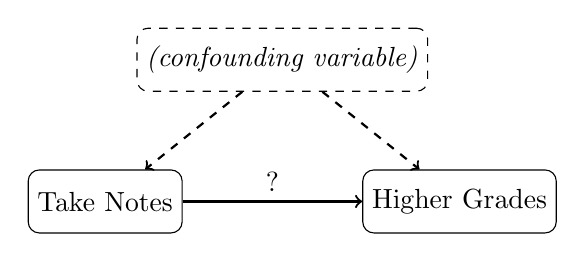
\begin{tikzpicture}[scale=0.9]
    % Nodes
    \node[draw, rounded corners, minimum width=1.8cm, minimum height=0.8cm] (notes) at (0,0) {Take Notes};
    \node[draw, rounded corners, minimum width=2cm, minimum height=0.8cm] (grades) at (5,0) {Higher Grades};
    \node[draw, rounded corners, minimum width=2.4cm, minimum height=0.8cm, dashed] (motivation) at (2.5,2) {\textit{(confounding variable)}};
    
    % Arrows
    \draw[->, thick] (notes) -- (grades) node[midway, above] {?};
    \draw[->, thick, dashed] (motivation) -- (notes);
    \draw[->, thick, dashed] (motivation) -- (grades);
\end{tikzpicture}
\end{center}
\vspace{0.3em}
\textbf{Fill in the confounding variable:} \blank{2in}
\end{tcolorbox}

\vspace{0.5em}

\subsection*{Part B: What Is an Experiment? \hfill \normalfont\small [3:32--5:43]}

\begin{enumerate}[label=\arabic*., leftmargin=2em, resume]
    \item An \textbf{experiment} is where a treatment or treatments are intentionally \blank{1.5in} on the experimental units.
    
    \vspace{0.3em}
    
    \item \textbf{Experimental units} are the \blank{1.75in} to which we apply the treatments. When experimental units are humans, we call them \blank{1.75in} or subjects.
    
    \vspace{0.3em}
    
    \item The \textbf{explanatory variable} (or \blank{1in}) may help to predict a change in the response variable.
    
    \vspace{0.3em}
    
    \item The \textbf{response variable} is what we use to \blank{1.5in} the outcome of a study.
    
    \vspace{0.3em}
    
    \item \textbf{Proposed experiment:} Let students \textit{decide} whether or not to take notes.
    \begin{itemize}[leftmargin=1.5em, topsep=2pt]
        \item Explanatory variable: Does the student take notes? (Levels: \blank{2in})
        \item Response variable: \blank{1.75in}
    \end{itemize}
    
    \vspace{0.3em}
    
    \item Is this a well-designed experiment? \hfill \textbf{Circle one:} \quad Yes \quad / \quad No
    
    \vspace{0.2em}
    
    \item Why or why not? Confounding is still possible because \blank{2.5in}.
\end{enumerate}

\vspace{0.4em}

\subsection*{Part C: Key Takeaways \hfill \normalfont\small [5:59--6:20]}

\begin{enumerate}[label=\arabic*., leftmargin=2em, resume]
    \item Observational studies cannot determine \blank{1.25in} due to possible \blank{1.25in}.
    
    \vspace{0.3em}
    
    \item An experiment intentionally imposes \blank{1.5in} on the participants in order to observe a \blank{1.5in}.
\end{enumerate}

\vspace{0.75em}

%==============================================================================
% VIDEO 2
%==============================================================================

\section*{\underline{Video 2}: Elements of a Well-Designed Experiment \hfill \normalfont\small [6:58]}

\subsection*{Part A: Four Principles of Experimental Design \hfill \normalfont\small [0:00--1:42]}

\begin{enumerate}[label=\arabic*., leftmargin=2em, start=15]
    \item A well-designed experiment must include:
    
    \vspace{0.5em}
    
    \begin{tabular}{|p{1.6in}|p{3.9in}|}
    \hline
    \textbf{Principle} & \textbf{Description} \\
    \hline
    & \\
    1. \blank{1.4in} & Compare at least \blank{0.5in} treatment groups (one could be a control group). \\
    & \\
    \hline
    & \\
    2. \blank{1.4in} & Randomly assign treatments to experimental units to balance out confounding factors. \\
    & \\
    \hline
    & \\
    3. \blank{1.4in} & Use \blank{1in} experimental units in each treatment group. \\
    & \\
    \hline
    & \\
    4. \blank{1.4in} & Control potential \blank{1.5in} where appropriate. \\
    & \\
    \hline
    \end{tabular}
\end{enumerate}

\vspace{0.5em}

\subsection*{Part B: Bulls-Eye! Example \hfill \normalfont\small [1:43--4:17]}

\begin{enumerate}[label=\arabic*., leftmargin=2em, resume]
    \item \textbf{Research question:} Does painting eyes on cattle's rears reduce \blank{1.5in}?
    
    \vspace{0.3em}
    
    \item A study in \blank{1.5in} randomly assigned cattle to receive one of three treatments:
    \begin{itemize}[leftmargin=1.5em, topsep=2pt]
        \item Treatment 1: \blank{1.5in} (683 cattle)
        \item Treatment 2: \blank{1.5in} (543 cattle)
        \item Treatment 3: \blank{1.5in} (835 cattle)
    \end{itemize}
    
    \vspace{0.3em}
    
    \item Results: Of the 683 cattle with eyespots, \blank{0.75in} were attacked. \blank{0.5in} cross-marked and \blank{0.5in} unmarked cattle were killed.
    
    \vspace{0.3em}
    
    \item This is an \blank{1.25in} (not observational) because cattle were \blank{1.5in} to treatments.
    
    \vspace{0.3em}
    
    \item How was \textbf{control} achieved in this study? The experiment was conducted in the same general \blank{1.25in} during the same general \blank{1.25in}.
\end{enumerate}

\vspace{0.5em}

\subsection*{Part C: Experimental Design Diagram \hfill \normalfont\small [4:18--6:27]}

\begin{enumerate}[label=\arabic*., leftmargin=2em, resume]
    \item Complete the experimental design diagram:
\end{enumerate}

\vspace{0.3em}

\begin{center}
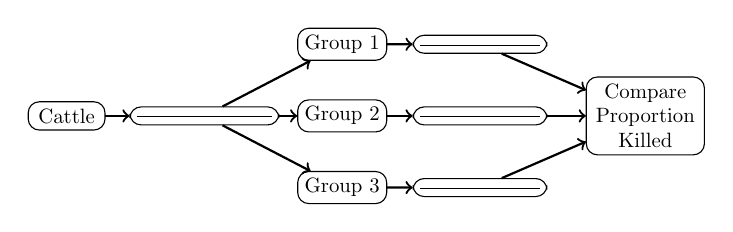
\begin{tikzpicture}[scale=0.7, every node/.style={scale=0.75}]
    % Starting node
    \node[draw, rounded corners, minimum width=1.3cm] (cattle) at (0,0) {Cattle};
    
    % Random allocation
    \node[draw, rounded corners, minimum width=1.8cm] (random) at (2.5,0) {\blank{0.9in}};
    
    % Groups
    \node[draw, rounded corners, minimum width=1.3cm] (g1) at (5,1.3) {Group 1};
    \node[draw, rounded corners, minimum width=1.3cm] (g2) at (5,0) {Group 2};
    \node[draw, rounded corners, minimum width=1.3cm] (g3) at (5,-1.3) {Group 3};
    
    % Treatments
    \node[draw, rounded corners, minimum width=1.3cm] (t1) at (7.5,1.3) {\blank{0.8in}};
    \node[draw, rounded corners, minimum width=1.3cm] (t2) at (7.5,0) {\blank{0.8in}};
    \node[draw, rounded corners, minimum width=1.3cm] (t3) at (7.5,-1.3) {\blank{0.8in}};
    
    % Compare
    \node[draw, rounded corners, minimum width=2cm, align=center] (compare) at (10.5,0) {Compare\\Proportion\\Killed};
    
    % Arrows
    \draw[->, thick] (cattle) -- (random);
    \draw[->, thick] (random) -- (g1);
    \draw[->, thick] (random) -- (g2);
    \draw[->, thick] (random) -- (g3);
    \draw[->, thick] (g1) -- (t1);
    \draw[->, thick] (g2) -- (t2);
    \draw[->, thick] (g3) -- (t3);
    \draw[->, thick] (t1) -- (compare);
    \draw[->, thick] (t2) -- (compare);
    \draw[->, thick] (t3) -- (compare);
\end{tikzpicture}
\end{center}

\vspace{0.4em}

\begin{enumerate}[label=\arabic*., leftmargin=2em, resume]
    \item \textbf{Important note:} On the AP Exam, simply providing a diagram may \textit{not} give full credit. You must also explain \blank{1in} the random assignment is performed.
    
    \vspace{0.3em}
    
    \item \textbf{One method:} Number all cattle from 1 to $N$. Use a \blank{2in} to select which cattle go to each group. Continue until the desired number are assigned to each treatment group.
\end{enumerate}

\vspace{0.5em}

\subsection*{Part D: Key Takeaways \hfill \normalfont\small [6:38--6:58]}

\begin{enumerate}[label=\arabic*., leftmargin=2em, resume]
    \item A well-designed experiment should include:
    \begin{itemize}[leftmargin=1.5em, topsep=2pt]
        \item \blank{1.5in} between at least two groups
        \item Random \blank{1.5in} of treatments to experimental units
        \item \blank{1.5in} of treatments to multiple experimental units
        \item \blank{1.5in} of possible confounding factors
    \end{itemize}
\end{enumerate}

\vspace{0.75em}

%==============================================================================
% VIDEO 3
%==============================================================================

\section*{\underline{Video 3}: Experimental Designs \& Methods \hfill \normalfont\small [10:11]}

\subsection*{Part A: Completely Randomized Design \hfill \normalfont\small [0:00--3:12]}

\begin{enumerate}[label=\arabic*., leftmargin=2em, start=27]
    \item \textbf{Example:} A melanoma treatment study compared standard care to a combination treatment. The \blank{2.25in} was measured in both groups.
    
    \vspace{0.3em}
    
    \item The study is described as: ``randomized, \blank{1.75in}, \blank{1.5in}''
    
    \vspace{0.3em}
    
    \item In a \textbf{completely randomized design}, treatments are assigned to experimental units completely at \blank{1in}.
    
    \vspace{0.3em}
    
    \item \textbf{Benefit:} Random assignment tends to \blank{1.5in} the effects of confounding variables so that differences in responses can be attributed to \blank{1.5in}.
    
    \vspace{0.3em}
    
    \item \textbf{Limitation:} Can \textit{all} differences in survival rate be attributed to the treatment? There may still be something about the \blank{1.25in} that affects results.
\end{enumerate}

\vspace{0.5em}

\subsection*{Part B: Randomized Block Design \hfill \normalfont\small [3:13--5:26]}

\begin{enumerate}[label=\arabic*., leftmargin=2em, resume]
    \item \textbf{Randomized Block Design} ensures that experimental units within each \blank{1in} are similar with respect to a blocking variable.
    
    \vspace{0.3em}
    
    \item Blocking helps to separate \blank{1.75in} from differences due to the blocking variable.
    
    \vspace{0.3em}
    
    \item In the melanoma study, \blank{1.75in} could be a blocking variable because the treatment may work differently for more severe vs.\ less severe cases.
    
    \vspace{0.3em}
    
    \item \textbf{Key distinction:} Blocking is \textbf{NOT} random. It's done by the \blank{1in}. Then, \textbf{within} each block, we \blank{1.1in}.
\end{enumerate}

\vspace{0.4em}

\begin{tcolorbox}[colback=white, colframe=apblue, boxrule=1pt, title={\textbf{Randomized Block Design Diagram}}]
\begin{center}
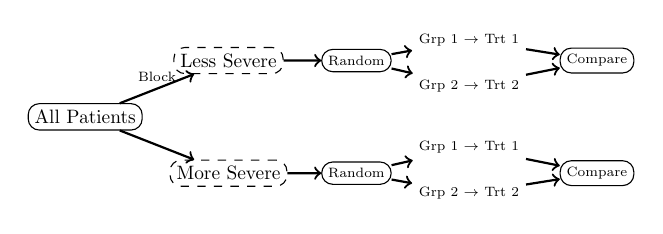
\begin{tikzpicture}[scale=0.65, every node/.style={scale=0.7}]
    % All patients
    \node[draw, rounded corners] (all) at (0,0) {All Patients};
    
    % Blocks
    \node[draw, rounded corners, dashed] (less) at (2.8,1.1) {Less Severe};
    \node[draw, rounded corners, dashed] (more) at (2.8,-1.1) {More Severe};
    
    % Random within blocks
    \node[draw, rounded corners, font=\scriptsize] (r1) at (5.3,1.1) {Random};
    \node[draw, rounded corners, font=\scriptsize] (r2) at (5.3,-1.1) {Random};
    
    % Groups
    \node[font=\scriptsize] (g1a) at (7.5,1.5) {Grp 1 $\to$ Trt 1};
    \node[font=\scriptsize] (g1b) at (7.5,0.6) {Grp 2 $\to$ Trt 2};
    \node[font=\scriptsize] (g2a) at (7.5,-0.6) {Grp 1 $\to$ Trt 1};
    \node[font=\scriptsize] (g2b) at (7.5,-1.5) {Grp 2 $\to$ Trt 2};
    
    % Compare
    \node[draw, rounded corners, font=\scriptsize] (c1) at (10,1.1) {Compare};
    \node[draw, rounded corners, font=\scriptsize] (c2) at (10,-1.1) {Compare};
    
    % Arrows
    \draw[->, thick] (all) -- (less) node[midway, above, font=\scriptsize] {Block};
    \draw[->, thick] (all) -- (more);
    \draw[->, thick] (less) -- (r1);
    \draw[->, thick] (more) -- (r2);
    \draw[->, thick] (r1) -- (g1a);
    \draw[->, thick] (r1) -- (g1b);
    \draw[->, thick] (r2) -- (g2a);
    \draw[->, thick] (r2) -- (g2b);
    \draw[->, thick] (g1a) -- (c1);
    \draw[->, thick] (g1b) -- (c1);
    \draw[->, thick] (g2a) -- (c2);
    \draw[->, thick] (g2b) -- (c2);
\end{tikzpicture}
\end{center}
\end{tcolorbox}

\vspace{0.5em}

\subsection*{Part C: Placebo and the Placebo Effect \hfill \normalfont\small [5:27--7:38]}

\begin{enumerate}[label=\arabic*., leftmargin=2em, resume]
    \item A \textbf{placebo} is a ``\blank{0.75in}'' treatment that is similar to the treatment being tested.
    
    \vspace{0.3em}
    
    \item \textbf{Why use a placebo?} So that all patients behave the same way (e.g., come in at the same \blank{1.25in}) regardless of which group they're in.
    
    \vspace{0.3em}
    
    \item The \textbf{placebo effect} occurs when experimental units have a \blank{1.25in} to a placebo. This is a naturally occurring phenomenon.
    
    \vspace{0.3em}
    
    \item Using a placebo helps determine if an effect is truly due to the \blank{1.5in} or just from receiving \textit{some} treatment.
\end{enumerate}

\vspace{0.5em}

\subsection*{Part D: Blinding \hfill \normalfont\small [7:39--8:13]}

\begin{enumerate}[label=\arabic*., leftmargin=2em, resume]
    \item \textbf{Single-blind experiment:} The \blank{1.25in} do not know which treatment they're receiving, but the researchers do (or vice versa).
    
    \vspace{0.3em}
    
    \item \textbf{Double-blind experiment:} Neither the \blank{1.25in} nor the \blank{1.5in} who interact with them know which treatment is being administered.
\end{enumerate}

\vspace{0.5em}

\subsection*{Part E: Matched Pairs Design \hfill \normalfont\small [8:14--9:28]}

\begin{enumerate}[label=\arabic*., leftmargin=2em, resume]
    \item \textbf{Matched Pairs Design} is a special type of block design where each block has size \blank{0.5in}.
    
    \vspace{0.3em}
    
    \item Pairs are arranged such that the two units are very closely \blank{1.25in} on relevant factors (like twins!).
    
    \vspace{0.3em}
    
    \item Within each pair, \blank{1.75in} is used to determine which unit receives which treatment.
    
    \vspace{0.3em}
    
    \item \textbf{Alternate form:} Each subject may receive \blank{1.25in}, with randomization to determine the \blank{1in} of treatments.
\end{enumerate}

\vspace{0.5em}

\subsection*{Part F: Key Takeaways \hfill \normalfont\small [9:29--10:11]}

\begin{enumerate}[label=\arabic*., leftmargin=2em, resume]
    \item A completely randomized design helps to \blank{1.5in} potential confounding variables.
    
    \item Block design ensures \blank{1.5in} within blocks \textit{before} randomization of treatments.
    
    \item The use of a \blank{1.25in} helps determine if an effect is truly due to the treatment.
    
    \item \blank{1.25in} occurs when subjects and/or researchers are unaware of the treatment.
\end{enumerate}

\vspace{0.75em}

%==============================================================================
% POST-VIDEO REFLECTION
%==============================================================================

\section*{Post-Video Reflection}

\begin{enumerate}[label=\arabic*., leftmargin=2em, start=49]
    \item \textbf{Identifying Components:} A pharmaceutical company wants to test whether a new pain medication is more effective than a current medication. They randomly assign 200 patients with chronic back pain to receive either the new medication or the current medication for 4 weeks, then measure pain levels.
    
    \vspace{0.3em}
    
    \begin{itemize}[leftmargin=1.5em]
        \item Experimental units: \blank{3in}
        \vspace{0.3em}
        \item Explanatory variable (factor): \blank{3in}
        \vspace{0.3em}
        \item Treatments: \blank{3in}
        \vspace{0.3em}
        \item Response variable: \blank{3in}
    \end{itemize}
    
    \vspace{0.5em}
    
    \item \textbf{Design Improvement:} The company is concerned that the severity of back pain (mild vs.\ severe) might affect how well the medication works. What type of experimental design would address this concern, and how would it be implemented?
    
    \vspace{1in}
    
    \item \textbf{Critical Distinction:} Explain the difference between \textbf{random selection} and \textbf{random assignment}. Which one allows us to generalize results? Which one allows us to establish causation?
    
    \vspace{1.1in}
    
    \item \textbf{Confounding Check:} A researcher wants to determine if drinking coffee improves test scores. She surveys students about their coffee habits and compares their exam grades. Identify one potential confounding variable and explain why it creates a problem.
    
    \vspace{1in}
\end{enumerate}

\vspace{0.5em}

%==============================================================================
% EXIT TICKET
%==============================================================================

\begin{tcolorbox}[colback=lightgray, colframe=apblue, boxrule=1.5pt, title={\textbf{Exit Ticket}}]
In 2--3 sentences, explain why random assignment of treatments is essential for establishing a cause-and-effect relationship.

\vspace{0.9in}
\end{tcolorbox}

\end{document}
